% nota teorica

%%  incluir la informaci´on del microcontrolador(caracter´ısticas generales, diagrama de bloques, diagrama de pines y características eléctricas), perifricos utilizados (esto incluye descripción de registros e instrucciones seg´un aplique), componentes electrónicos complementarios; as´ı como también el diseño del circuito justificando los valores o función de los componentes electrónicos/digitales utilizados (debe incluir una lista de la cantidad de componentes y sus precios) e información de los conceptos fundamentales adicionales que se ven en clase

%informacion general mcu 
\subsection{Información general del Arduino Nano 33 BLE}


    %caracteristicas 
    \subsubsection{Características}

    Los microcontroladores utilizados en las placas Arduino están integrados en miles de millones de dispositivos de uso cotidiano, un ejemplo son los dispositivos \textit{wearables} (en inglés), o bien, usables, ponibles. También, otros ejemplos son los drones, impresoras 3D, juguetes, arroceras, enchufes inteligentes y lavadoras, entre otros. Estos MCU de bajo costo buscan hacer más accesible el IoT. \cite{arduino}. Este MCU se configura a partir de la plataforma de código abierto llamada Arduino. Asimismo, el MCU de la placa Arduino Nano BLE 33 se trata de un Arm Cortex-M4 que funciona a 64 MHz, con 1 MB de memoria Flash y 256 KB de RAM. \cite{arduino}



    
    %diagrama de bloques 
    \subsubsection{Diagrama de bloques}
    Se muestra el diagrama de bloques MCU: 

    \begin{figure}[H]
        \centering
        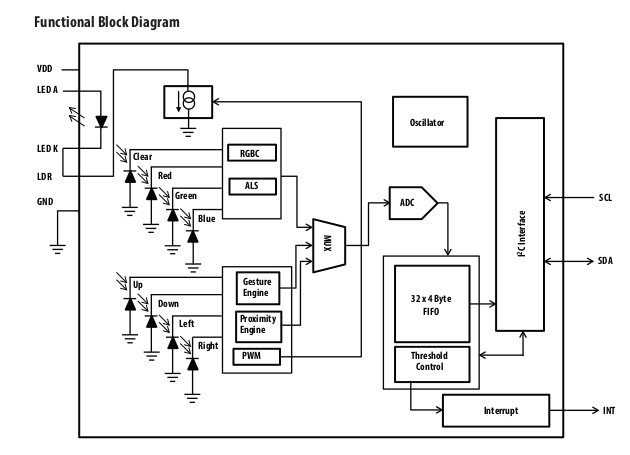
\includegraphics[width=0.8\linewidth]{pics/diagrama_bloque.png}
        \caption{Diagrama de bloques para el Arduino Nano 33 BLE}
        \label{fig:bloque}
    \end{figure}
    
    %diagrama de pines 
    \subsubsection{Diagrama de pines}

    A continuación se muestra el diagrama de pines del Arduino Nano 33 BLE obtenido de la hoja de datos: 

    \begin{figure}[H]
        \centering
        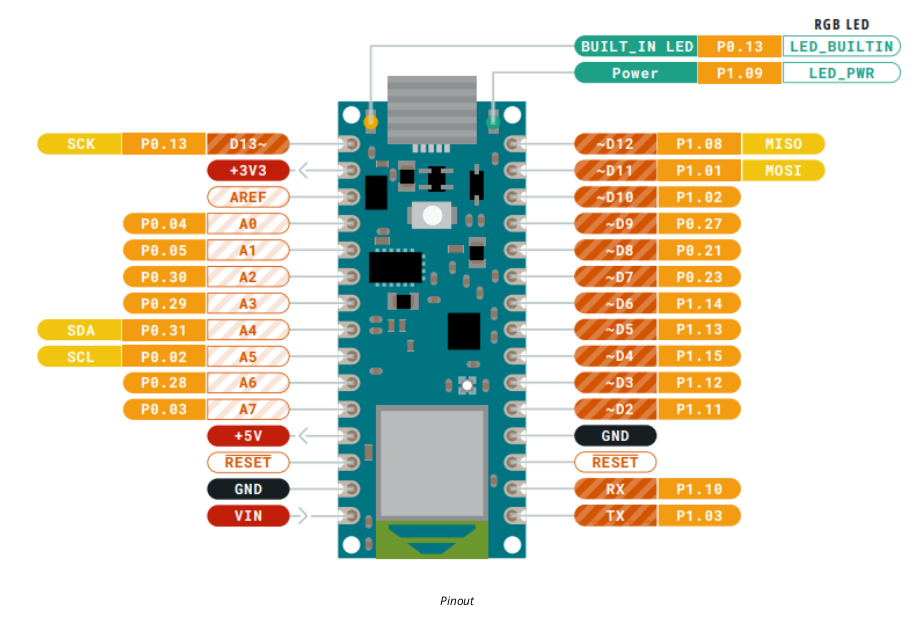
\includegraphics[width=0.8\linewidth]{pics/diagrama_pin.png}
        \caption{Diagrama de pines para el Arduino Nano 33 BLE}
        \label{fig:pin}
    \end{figure}

    \begin{figure}[H]
        \centering
        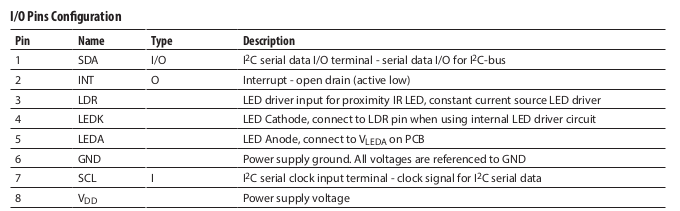
\includegraphics[width=0.8\linewidth]{pics/pines.png}
        \caption{Especificaciones de los pines para el Arduino Nano 33 BLE}
        \label{fig:pines}
    \end{figure}
    
    %caracteristicas electricas
    \subsection{Características eléctricas}
    
    \begin{figure}[H]
        \centering
        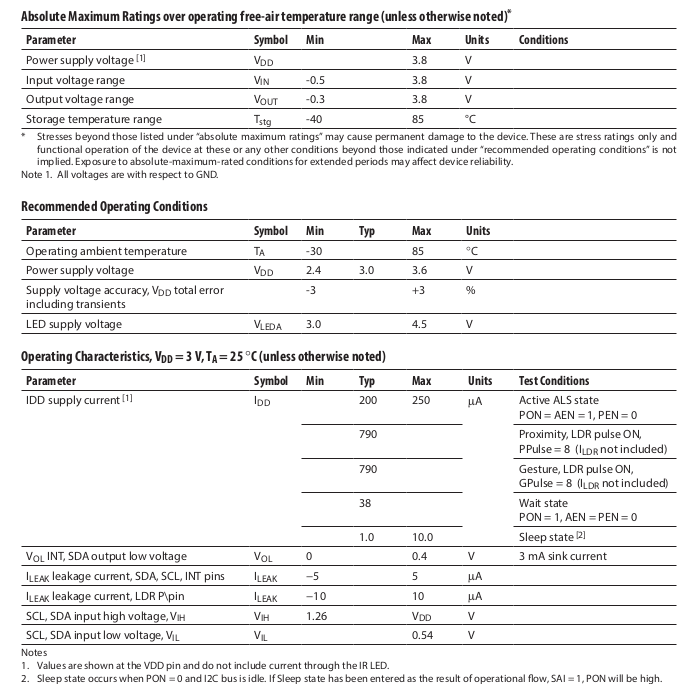
\includegraphics[width=0.8\linewidth]{pics/electricas.png}
        \caption{Especificaciones eléctricas el Arduino Nano 33 BLE}
        \label{fig:electricas}
    \end{figure}

%%%%%%%%%%%%%%%%%%%%%%%%%%%%%%%%%%%%%%%%%%%%%%%%%%%%
%%%%%%%%%%%%%%%%%%%%%%%%%%%%%%%%%%%%%%%%%%%%%%%%%%%%

%• Periféricos
\subsection{Periféricos}

%descripción de registros e instrucciones

Se utilizan los periféricos utilizados son el acelerómetro y el giroscopio integrados en el Arduino Nano 33 BLE, donde estos sensores son parte del módulo LSM9DS1 y con los cuales se permite medir la aceleración y la orientación angular. \\

%%%%%%%%%%%%%%%%%%%%%%%%%%%%%%%%%%%%%%%%%%%%%%%%%%%%
%%%%%%%%%%%%%%%%%%%%%%%%%%%%%%%%%%%%%%%%%%%%%%%%%%%%

%• Diseño de circuito
\subsection{Diseño de circuito}

En la figura \ref{diseno}, se aprecia la placa Arduino Board Nano 33 BLE Sense Lite montada en una placa extra para facilidad. También, un cable USB está transmitiendo la información hacia la PC y viceversa. Entonces, el diseño es simple en términos de la electrónica empleada; la mayor parte de la elaboración del laboratorio se llevo a cabó en programación. 

    \begin{figure}[H]
        \centering
        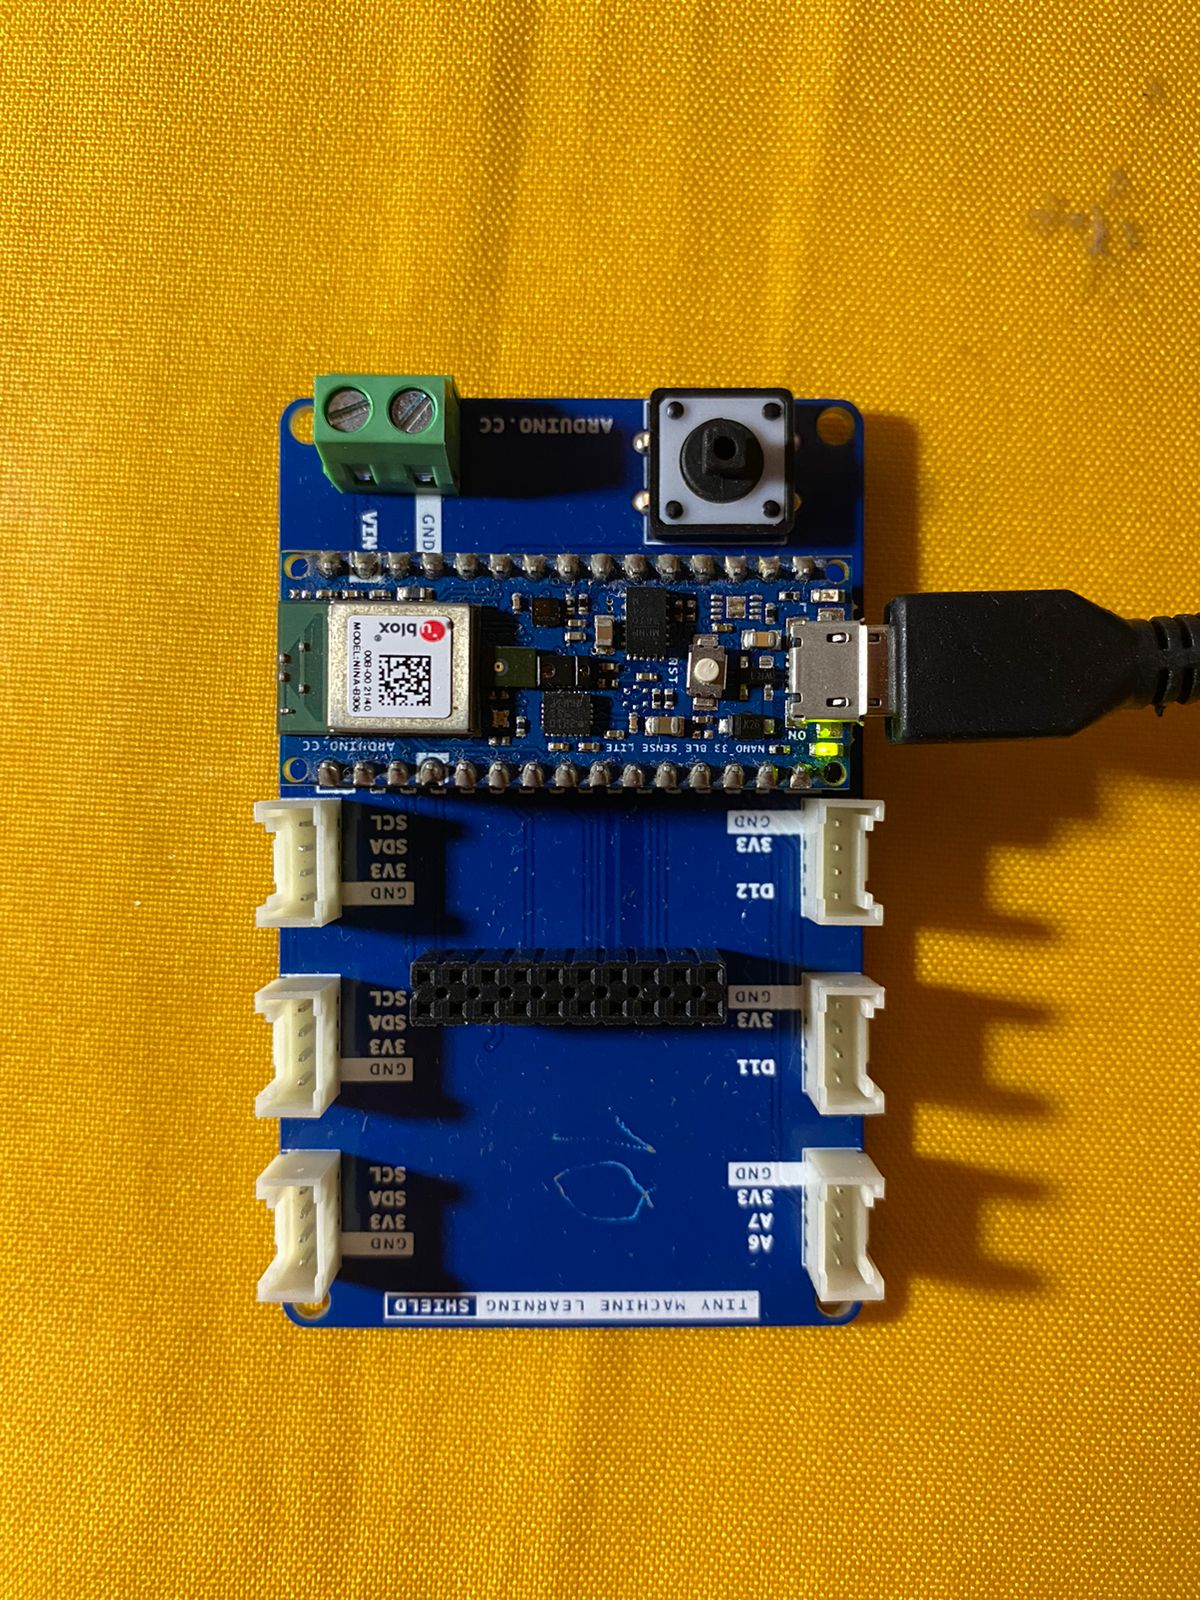
\includegraphics[width=0.5\linewidth]{pics/diseno.jpeg}
        \caption{Diseño del circuito electrónico.}
        \label{diseno}
    \end{figure}

%%%%%%%%%%%%%%%%%%%%%%%%%%%%%%%%%%%%%%%%%%%%%%%%%%%%
%%%%%%%%%%%%%%%%%%%%%%%%%%%%%%%%%%%%%%%%%%%%%%%%%%%%

%• Lista de componentes y precios
\subsection{Lista de componentes y precios}

\begin{table}[H]
\centering
\begin{tabular}{ll}
\hline
\multicolumn{1}{|c|}{Componente}          & \multicolumn{1}{c|}{Precio en colones} \\ \hline
\multicolumn{1}{|c|}{Arduino Nano 33 BLE Sense Lite} & \multicolumn{1}{c|}{23 000}            \\ \hline

\end{tabular}
\end{table}

%%%%%%%%%%%%%%%%%%%%%%%%%%%%%%%%%%%%%%%%%%%%%%%%%%%%
%%%%%%%%%%%%%%%%%%%%%%%%%%%%%%%%%%%%%%%%%%%%%%%%%%%%

